% !TEX root = ../PhD Thesis.tex
\chapter{Introduction}
\pagenumbering{arabic}

\section{The origin of life}

To follow my work, we have to rewind back some years ago. Millions and millions of years ago.
Once upon a time there was a violent, harsh and unwelcoming planet among countless others. Earth was lifeless. But as millions of years went by, it started being home to a complex recipe whose special sauce is still being studied to this day: the primordial soup \cite{gilbert:1986td}. These were the perfect conditions for a young, 500-million-year-old planet to brew life.

And what is life? Although this question is not easy to answer, we know that living organisms as we know them are complex, carbon-based systems composed of nucleic acids, proteins, carbohydrates and lipids. Together with some smaller molecules, these are known as biomolecules and are crucial for the survival of living organisms \cite{alberts:2008vj}.

Amongst those biomolecules, my work focuses on two: proteins and nucleic acids. Proteins have many important functions in an organism, including catalysing chemical reactions (enzymes), signalling cellular processes (hormones) and playing a role in the immune system (antigens) \cite{alberts:2008vj}. Regarding nucleic acids, deoxyribonucleic acid (DNA) stores the genetic data, the blueprint required to generate the majority of the vital molecules in the cell, including ribonucleic acid (RNA) molecules for protein synthesis and regulation \cite{alberts:2008vj}.
% messenger RNAs (mRNA) are coding RNAs whose sequence is used as a template to create new proteins, transfer RNAs (tRNA) carry amino acids to generate proteins and ribosomal RNAs (rRNA) are the major components of the ribosome, the protein synthesis machinery. Other non-coding RNAs (long non-coding RNAs, small interfering RNAs, micro RNAs, etc.) have further regulatory roles in the cell.

% Miller-Urey experiment
% But how did all this complexity emerged from the primordial soup? The primitive Earth's  atmosphere was rich in inorganic compounds (the exact ones are still up to debate). Together with 

One possibility for the origin of life is based on the \emph{RNA world}, an hypothesis that states that primitive life forms were based on self-replicating RNA that predates DNA and proteins in evolution \cite{gilbert:1986td,alberts:2008vj,sharp:1985th}. After all, those RNA molecules could store genetic information like DNA and catalyse chemical reactions akin to enzymes, making RNA a prime candidate for life to take its first steps. As life evolved, these specific catalysing and storing functions may have been overtaken by protein enzymes that were more effective as reaction catalysers, and DNA, a more stable and less error-prone nucleic acid to store genetic information \cite{gilbert:1986td,alberts:2008vj}.

% Many discoveries were made that led to this hypothesis of the RNA world and of RNA as the main molecule responsible for the first life forms: from discovering the nucleic acids

% Re-creating the RNA world, 1995 review, https://www.cell.com/action/showPdf?pii=S0960-9822%2895%2900205-3

% Progenote: the last common ancestor of modern life

% Gene expression

\section{Nucleic acids and protein synthesis}

The word \emph{protein} was first used in a publication by Gerardus Mulder in 1838, following the suggestion by his colleague Jöns Berzelius. In his publication almost two centuries apart from today, Mulder reported the chemical compounds of \emph{les substances les plus essentielles du règne animal: la fibrine, l'albumine et la gélatine} \cite{mulder:1838uy}. % we owe to Berzelius in his later years not only the generalizations which he crystallized in the words 'isomerism', 'polymerism' and 'catalysis'
To refer to these substances, Mulder named these words \emph{protein} based on a Greek adjective that means of the \emph{first rank or position}, reflecting the perceived importance of those molecules \cite{mulder:1838uy,vickery:1950ur}.

% Mendel?

Some decades later in 1869, Friedrich Miescher isolated a mysterious, protein-like substance from the pus of fresh surgical bandages that he named \emph{nuclein}, found to be present in the cell nucleus of diverse animals, plants and fungi. Miescher's work led him to believe that increased nuclein could be associated with the first stages of cell division in proliferating tissues \cite{dahm:2005wx}. Albrecht Kossel (a former professor of Miescher) and colleagues described 5 organic compounds from nuclein: adenine, cytosine, guanine, thymine, and uracil \cite{kossel:1885tj,kossel:1893ws,kossel:1894vy,ascoli:1901ti}. Nuclein was eventually renamed \emph{nucleic acid}, but its importance was not recognised at the time \cite{dahm:2005wx}.

% 1880: coined "mutation"

% Around the 1900s, the physician Archibald Garrod studied peculiar cases of metabolic diseases that he later proposed to be related with hereditary defects, based on Mendel's laws of inheritance, publishing the first recorded cases of genetic disorders in humans in the book \emph{Inborn Erros of Metabolism} \cite{}.

% In 1909, the botanist Johannsen coined the terms \emph{gene} and \emph{phene}, \emph{genotype} and \emph{phenotype}. % confirm about "phene"

In the first decades of the 20th century, the scientific consensus was that proteins carried genetic information, but Boveri and Sutton theorised otherwise \cite{dahm:2005wx,sutton:1902tx}:

\begin{displayquote}[\cite{sutton:1902tx}]
the association of paternal and maternal chromosomes in pairs and their subsequent separation during the reducing division (...) may constitute the physical basis of the Mendelian law of heredity.
\end{displayquote}

%\begin{figure}[!h]
%  \vspace{-\intextsep}
%  \centering
%  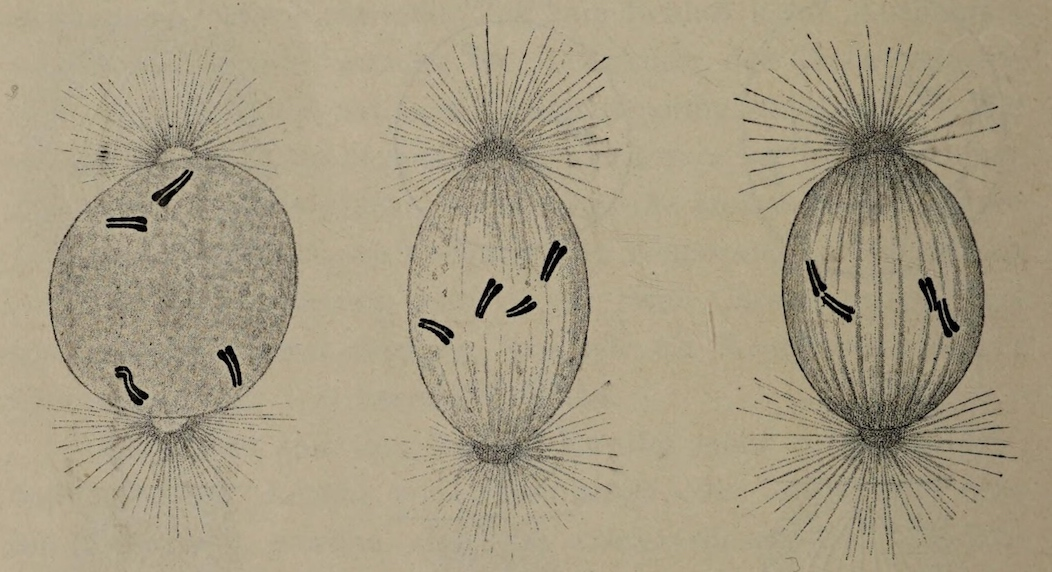
\includegraphics[width=.5\linewidth]{images/intro/boveri-sutton-cropped}
%  \caption[Chromosome segregation during egg maturation in \emph{Ophryotrocha}]{\textbf{Chromosome segregation during egg maturation in \emph{Ophryotrocha}}.}
  % source: https://wellcomecollection.org/works/an45kexq/items?canvas=76
  % Ergebnisse über die Konstitution der chromatischen Substanz des Zellkerns / von Theodor Boveri.. Public Domain Mark
%\end{figure}

\begin{wrapfigure}{r}{.35\textwidth}
  \vspace{-\intextsep}
  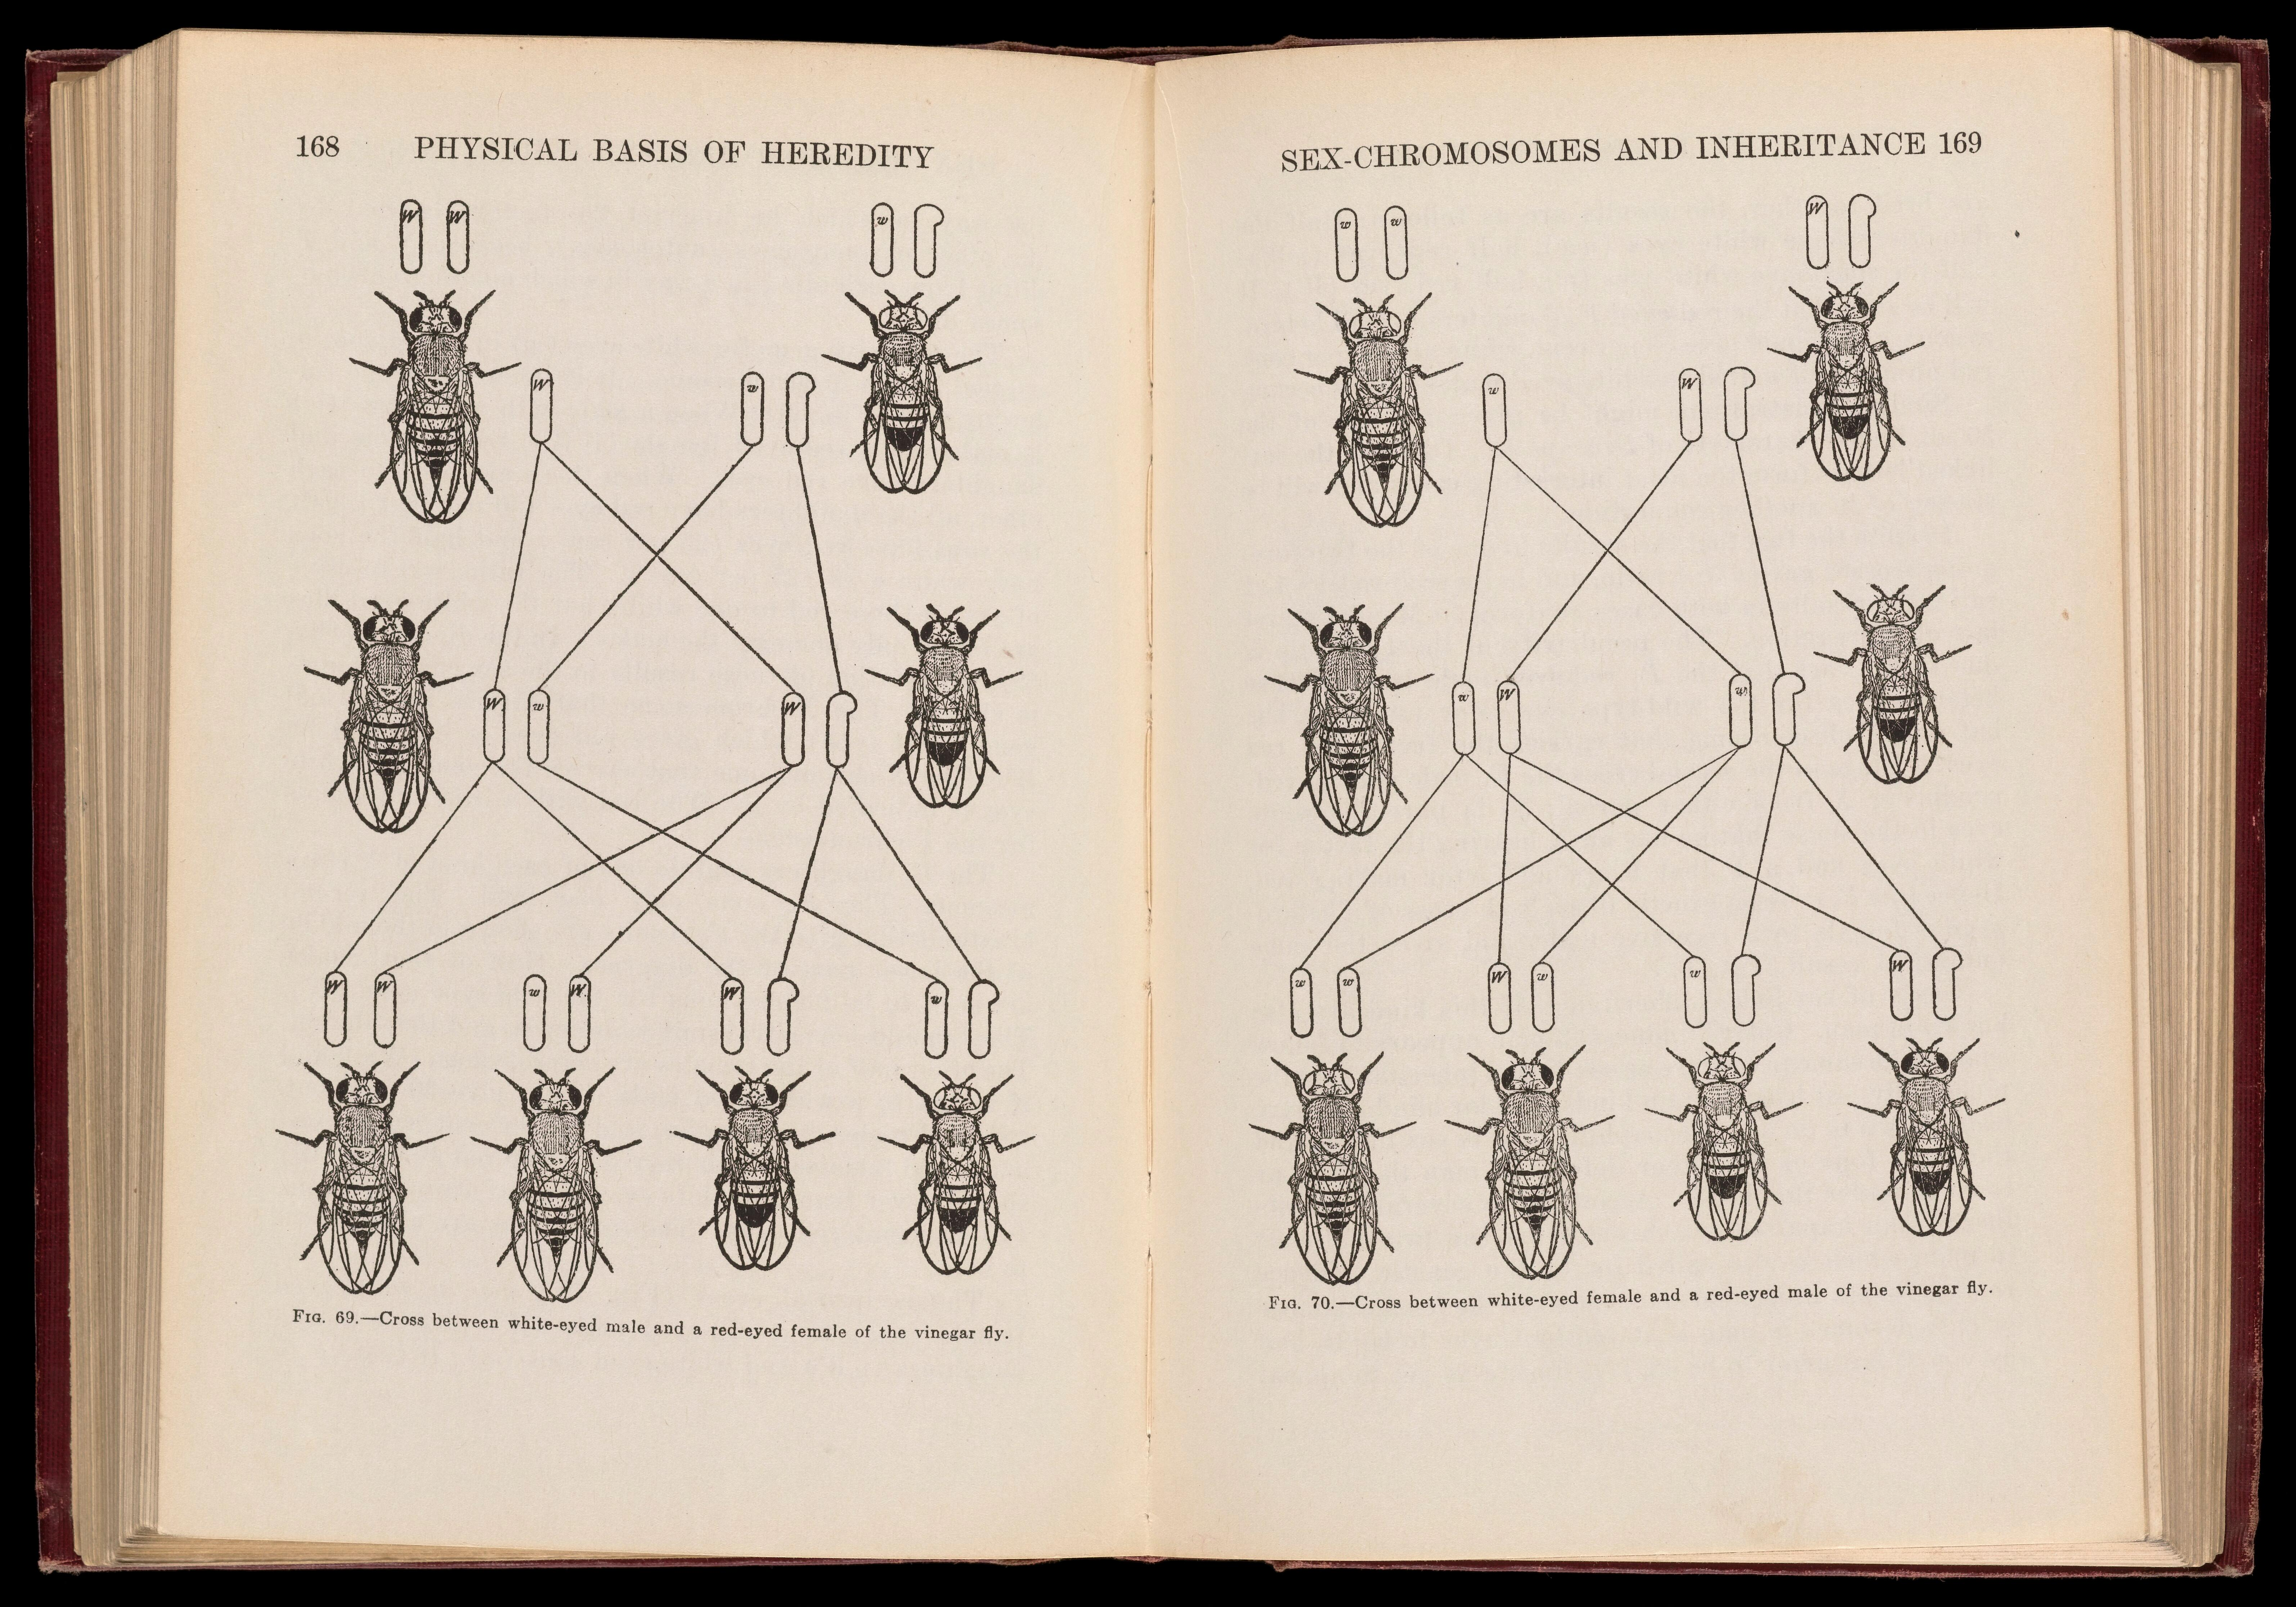
\includegraphics[width=\linewidth]{images/intro/thomas-morgan-fly}
  \caption[Thomas Morgan's fruit fly experiments]{\textbf{Thomas Morgan's fruit fly experiments}.}
  \vspace{-\intextsep}
  % source: https://wellcomecollection.org/works/k3rwcqc3/images?id=ey2zux4q
\end{wrapfigure}

The Boveri-Sutton chromosome theory of genetic inheritance followed Mendel's controversial \cite{} work from 1865 \cite{sutton:1902tx} and was later supported by fruit fly experiments from an initially skeptical \cite{} Thomas Morgan \cite{morgan:1915tw}. In 1915, Thomas Morgan, Hermann Muller and colleagues published a textbook with their findings describing genetic dominance, sex inheritance and chromosomal crossover. One chapter was provokingly titled \emph{The Chromosomes as Bearers of Hereditary Material} \cite{morgan:1915tw}. In 1927, Hermann Muller discussed that exposure of fruit flies to X-ray radiation induced hundreds of genetic mutations, greatly contributing to the study of genetic mutations and evolution \cite{muller:1927wl} \footnote{Muller's 1927 Science paper \cite{muller:1927wl} that earned him the Nobel prize was not peer-reviewed, cited no references and lacked the methods section \cite{calabrese:2018vl}. This may have happened not only because Muller wanted to be the first to share his hypothesis, but also because he agreed with the criticism by his long-time friend Edgar Alternburg that believed his data was not strong enough to confirm the induction of mutations \cite{calabrese:2018vl}. It would take until 1930 for Muller to publish results addressing Altenburg's criticism, although Muller was aware of the issues before 1927 \cite{calabrese:2018vl}.}.

% 1928: Frederick Griffith postulates that a "transforming principle" permits properties from one type of bacteria (heat-inactivated virulent Streptococcus pneumoniae) to be transferred to another (live nonvirulent Streptococcus pneumoniae).

At the time, nucleic acids were classified as \emph{thymus nucleic acid} found in animals (specially enriched in the thymus, hence its name) and \emph{yeast nucleic acid} found in plants\footnote{\emph{Yeast nucleic acid} was so named since first extracted from yeasts, considered from the plant kingdom by most scientists at the time. Starting with Ernst Haeckel in 1878, alternative proposed systems clumped fungi together with unicellular organisms instead (kingdoms of Protoctista, Protista, etc.) \cite{haeckel:1878tz}. In 1959, Robert Whitakker suggested a fungi kingdom amid three others \cite{whittaker:1959to}, a proposal that later blossomed into his popular five-kingdom classification system published in 1969 \cite{whittaker:1969to}. In his 1969 article, Whittaker explains why fungi should not be considered plants to his fellow peers.}. However, in 1933, Jean Brachet found evidence of \emph{thymus nucleic acid} in the cell nucleus and of \emph{yeast nucleic acid} in the cytoplasm of eukaryotic cells. His work suggested that both types of nucleic acids were present in the same cell with potentially different roles. During the 1930s, Phoebus Levene identified the phosphate backbone of nucleic acids, including its pentose sugars (deoxyribose and ribose) \cite{levene:1929ug}, which inspired their contemporary nomenclature: \emph{thymus nucleic acid} is now known as deoxyribonucleic acid (DNA) and \emph{yeast nucleic acid} as ribonucleic acid (RNA).
% confirm if in this Levene paper

Although the word \emph{gene} was used since 1909 to abstractly refer to Mendelian factors of inheritance (i.e. the units of heredity) \cite{}, Demerec tried to define it in his 1933 publication, \emph{What is a Gene?}, alongside a figure of the \emph{tentative structure of thymus nucleic acids} (DNA):

\begin{displayquote}[\cite{demerec:1933td}]
(...) [A gene] is a minute organic particle, capable of reproduction, located in a chromosome and responsible for the transmission of a hereditary characteristic.
\end{displayquote}

Later in 1941, Edward Tatum and George Beadle hypothesised that each gene is responsible for producing a specific enzyme and demonstrated that radiation-induced mutations could alter the resulting enzyme \cite{beadle:1941vs}. Together with Joshua Lederberg, Tatum demonstrated in 1946 that bacteria can exchange genetic material in a process called genetic recombination \cite{lederberg:1946wl}.

% 1940s, 50s: mobile genetic elements, Barbara McClintock

% 1960s, it was shown in work done in the laboratories of Werner Arber and Matthew Meselson that the restriction is caused by an enzymatic cleavage of the phage DNA, and the enzyme involved was therefore termed a restriction enzyme.
% The 1978 Nobel Prize for Physiology or Medicine was awarded to Werner Arber, Daniel Nathans, and Hamilton O. Smith.[23] The discovery of restriction enzymes allows DNA to be manipulated, leading to the development of recombinant DNA technology that has many applications, for example, allowing the large scale production of proteins such as human insulin used by diabetic patients

\begin{wrapfigure}{R}{.45\textwidth}
  \vspace{-\intextsep}
  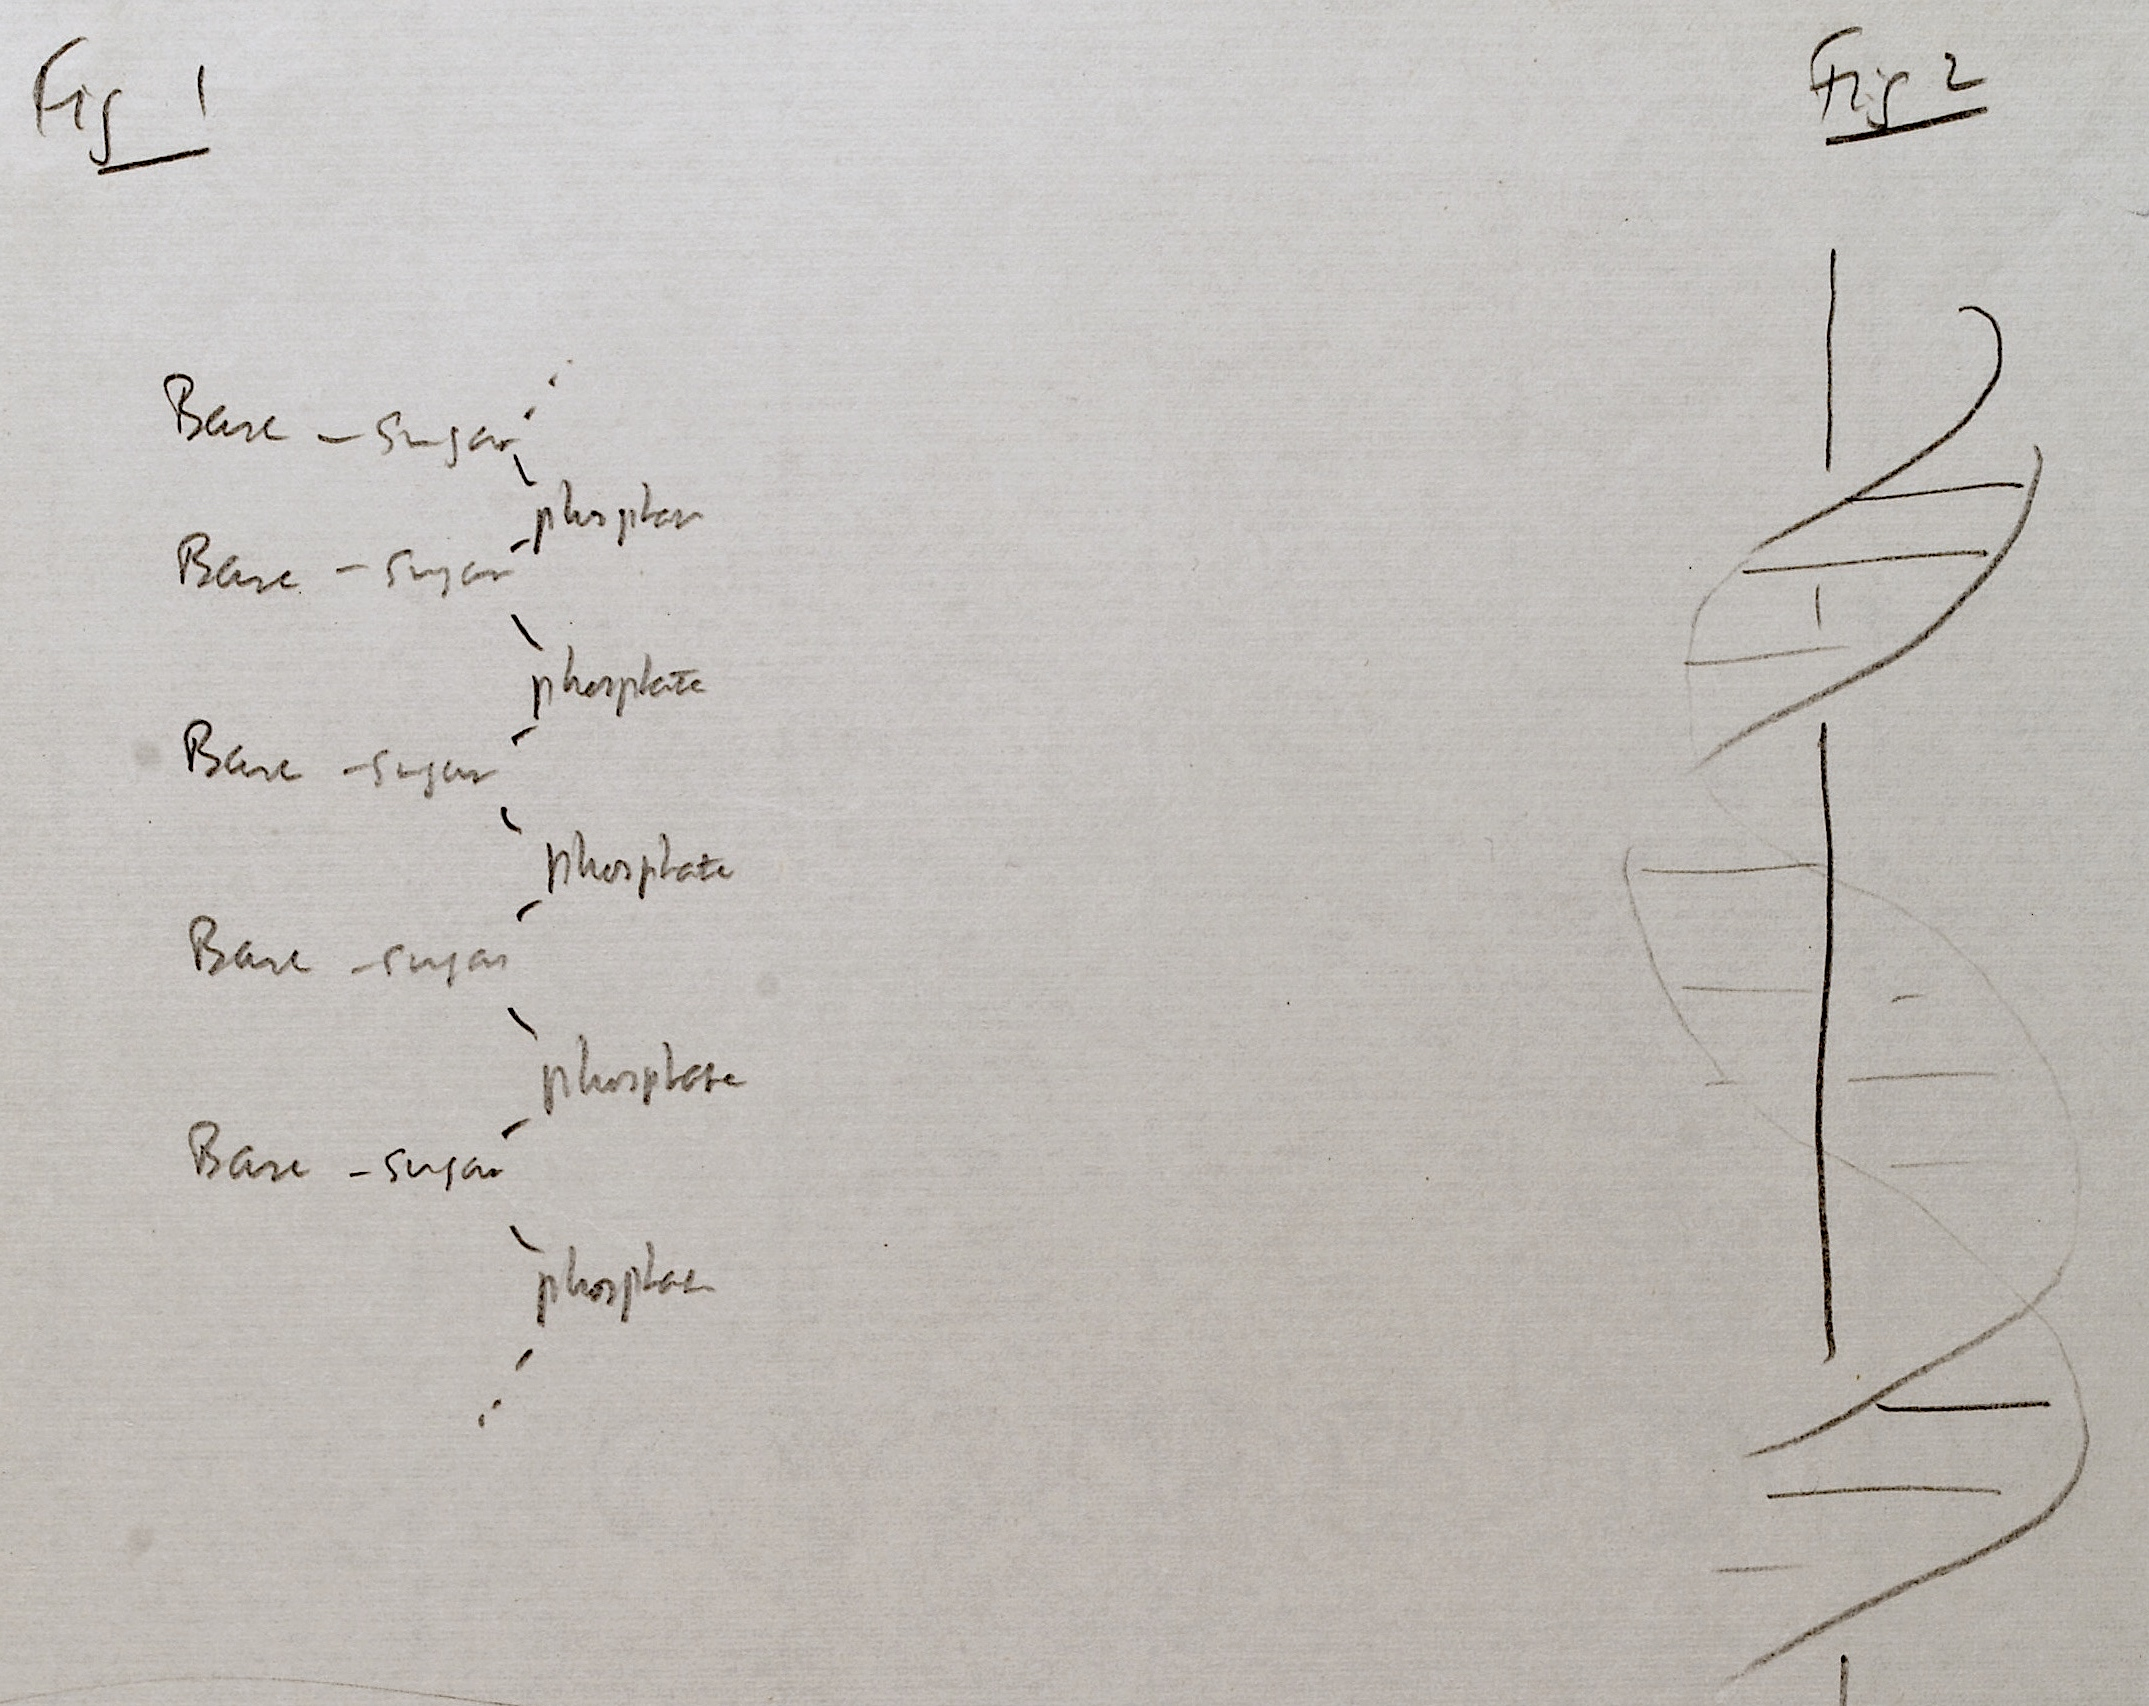
\includegraphics[width=\linewidth]{images/intro/dna_structure_draft_cropped}
  \caption[Figure drafts for a manuscript on DNA structure]{\textbf{Figure drafts for a manuscript on DNA structure from Francis Crick and James Watson}.}
  \label{fig:dna-structure}
  \vspace{-\intextsep}
\end{wrapfigure}

In 1952, Alfred Hershey and Martha Chase demonstrated that during viral infection by bacteriophage T2, its DNA, but not any viral protein, enters inside the bacteria \cite{hershey:1952wo}. The viral DNA is enough to produce the DNA molecules found in progeny virus particles. Amid the contemporary belief that proteins were the carriers of hereditary information, the Hershey-Chase experiment complemented previous publications suggesting that that role belonged to DNA \cite{hershey:1952wo}.

The work by Rosalind Franklin and Maurice Wilkins on analysing DNA using X-ray crystallography was crucial to the discovery of DNA's double helix structure, published in 1953 by Francis Crick and James Watson \cite{watson:1953ug}. DNA is composed by two phosphate-sugar chains linked together via hydrogen bonds by pairs of nucleotides: adenine pairs with thymine and cytosine with guanine. Crick and Watson also proposed that this strand complementarity could be important for DNA replication \cite{watson:1953ug}. Afterwards, Arthur Kornberg observed the proposed nucleotide pairing in DNA synthesised by an enzyme that replicates DNA using one of its strands as a template: the DNA polymerase \cite{kornberg:1956wk}.

During a time when not all scientists agreed that nucleic acids played a role in protein synthesis, George Palade described in 1955 the ribosome as \emph{a small particulate component of the cytoplasm} that associates with RNA in the endoplasmic reticulum membrane to perform protein synthesis \cite{palade:1955tf,jacob:1961uh}. The associated RNA was identified as of two types: ribosomal RNA (rRNA) that composed the ribosome itself and \emph{soluble RNA} -- transfer RNA (tRNA) --, found to carry the amino acids for protein synthesis \cite{hoagland:1958vm,jacob:1961uh}. Multiple ribosomes were found to bind to a single RNA molecule (polysomes), allowing for parallelised protein synthesis \cite{warner:1963uj}.

\begin{wrapfigure}{l}{.35\textwidth}
  \vspace{-\intextsep}
  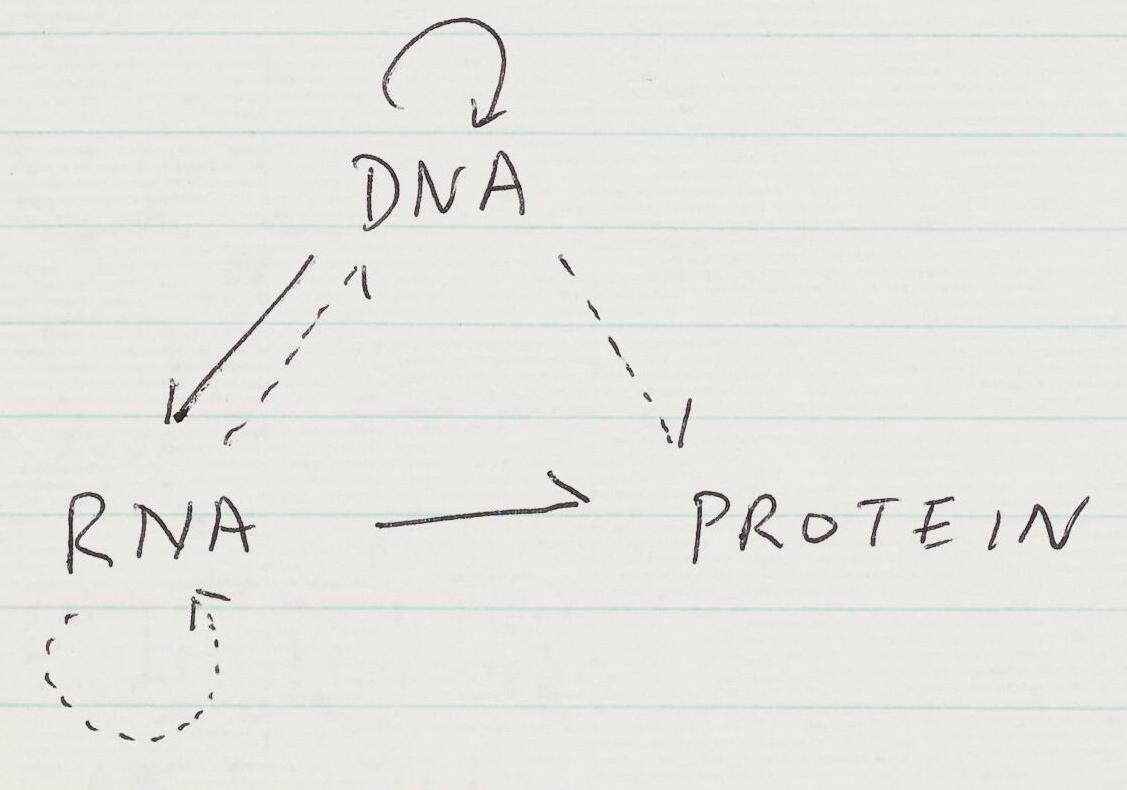
\includegraphics[width=\linewidth]{images/intro/crick-central-dogma cropped}
  \caption[Central dogma of molecular biology]{\textbf{Central dogma of molecular biology} as drafted by Francis Crick.}
  \label{fig:central-dogma}
  \vspace{-\intextsep}
  % https://wellcomecollection.org/works/ntzhcpgg/items?canvas=51
\end{wrapfigure}

Piece by piece, the role of DNA and RNA in protein synthesis was becoming clearer. Francis Crick proposed in 1958 that the genetic information flows from DNA to protein via RNA: the \emph{central dogma of molecular biology}\cite{crick:1958ws,crick:1970aa}. It was also hypothesised at that time that triplets (\emph{codons}) of the four nucleotides found in nucleic acids were necessary to produce each of the 20 universally-found types of amino acids that compose a protein \cite{crick:1958ws,crick:1961ui} and that those amino acids would be responsible for the protein's three-dimensional structure -- and consequently, its functionality \cite{crick:1958ws}. It took less than a decade to unravel which codons code for which aminoacid, an important breakthrough that allowed to predict protein sequences from DNA and RNA via the so-called universal genetic code \cite{khorana:1966vr,crick:1968wg}. % universal to virtually all species
In 1959 and 1960, DNA-dependent RNA polymerase, an enzyme that synthesises RNA from DNA and common to all living organisms, was independently described by the labs of Samuel Weiss, Jerard Hurwitz and Audrey Stevens \cite{hurwitz:1960uf,weiss:1959vp,stevens:1960ue} \footnote{In 1955, Severo Ochoa and Marianne Grunberg-Manago discovered the polynucleotide phosphorylase (PNPase) enzyme that they thought to synthesise RNA polymers from DNA \cite{grunberg-manago:1956wb}. Ochoa was erroneously awarded a Nobel prize in 1959 for discovering the biological mechanism of RNA synthesis \cite{}.}.

% RNA structure?
% Doty, P., Boedtker, H., Fresco, J.R., Haselkorn, R. and Litt, H. (1959) PNAS 45, 482-498. 10
% Fresco, J.R., Alberts, B.M. and Doty, P. (1960) Nature 188, 98-101.

François Jacob and Jacques Monod speculated in 1961 that ribosomal protein synthesis required an intermediate molecule with the template message to convert from DNA to protein and that would act as the \emph{messenger} \cite{jacob:1961uh,brenner:1961ve}. Unlike many of their contemporaries, they dismissed the known rRNA (and tRNA) molecules as the template for protein synthesis, given that they did not reflect the base composition of DNA, among other properties \cite{jacob:1961uh}. Based on contemporary experiments, Jacob and Monod proposed unstable RNA molecules as relevant candidates and named them messenger RNA (mRNA) \cite{jacob:1961uh,brenner:1961ve}. Making the distinction between \emph{structural genes} and \emph{other, functionally specialized, genetic determinants}, Jacob and Monod also discussed the induced activation of repressors in mRNA synthesis \cite{jacob:1961uh}.

In the 1969 publication entitled \emph{Gene Regulation for Higher Cells: A Theory}, Roy Britten and Eric Davidson proposed that:

\begin{displayquote}[\cite{britten:1969va}]
Cell differentiation is based almost certainly on the regulation of gene activity, so that for each state of differentiation a certain set of genes is active in transcription and other genes are inactive.
\end{displayquote}

Among the first publications of its kind, Britten and Davidson theorised about the intricate networks of gene regulation as fine-tuned systems in higher organisms based on the redundancy of different genomic elements and feedback loops. As they wrote, large genome sizes do not imply an increase in the number of genes compared to smaller genomes, but rather an increase in regulation complexity: \emph{a large amount of DNA [including repeated DNA sequences] could be devoted to regulatory function}, for instance by sequence-specific binding of RNA from another gene \cite{britten:1969va}. 

In the beginning of the 1970s, the first studies on RNA processing were published. At the time, two types of RNA were distinguished inside the nucleus: ribosomal precursor RNA molecules that yield cytoplasmic rRNA and heterogeneous nuclear RNA (hnRNA) whose composition \emph{resembles that of DNA} \cite{darnell:1971tg}. \emph{Polyadenylic acid} (polyA) sequences ranging from 150 to 250 nucleotides were found to be added to the 3$'$ end of hnRNAs and cytoplasmic mRNAs, the first sign of eukaryotic RNA processing \cite{darnell:1971tg,edmonds:1971vr}. James Darnell and colleagues thus proposed that hnRNAs and cytoplasmic mRNAs were related: the polyA sequence is added to hnRNAs post-transcriptionally in order to enable the export of nuclear RNAs to the cytoplasm, which are later found to be associated with ribosomes for protein synthesis \cite{darnell:1971tg,edmonds:1971vr}. Later in 1974, the addition of a 5$'$-methylated cap was found in hnRNA and cytoplasmic mRNA and was proposed as an eukaryotic post-transcriptional RNA modification that protects the 5$'$-end of RNAs from degradation enzymes \cite{perry:1974uj,rottman:1974tk}.
% Other functions of polyA tails and 5' cap?

% Most RNAs are non-coding: 97\% in eukaryotes?

% protein synthesis occurs in the cytoplasm
% RNA degradation?

% From the mid 1970s, through studies of bacteria, Tomas Lindahl showed how certain protein molecules, repair enzymes, remove and replace damaged parts of DNA. These discoveries have increased our understanding of how the living cell works, the causes of cancer and aging processes.

\subsection{Alternative splicing}

% A gene is a segment of DNA that is transcribed to RNA and, in case of mRNA, may later be encoded as a protein. The whole process from gene to its product is known as gene expression and summarises multiple, complex steps that occur within the cell to maintain its well-being. Such processes include RNA synthesis (transcription), RNA splicing and protein synthesis (translation).

% It was also Crick that suggested we would study evolution by comparing sequences across species.

First reported in mammalian cells infected with human adenovirus 2 \cite{berget:1977wp,chow:1977wn} and later observed in endogenous mammalian and eukaryotic genes \cite{brack:1977we,early:1980wq}, mRNA-DNA hybridisation experiments starting in 1977 suggested that genes are composed by intervening non-coding sequences, based on experiments from Richard Roberts, Philip Sharp and colleagues. During or after transcription of the precursor mRNA (pre-mRNA), non-coding sequences (introns) are excised from the transcript, remaining only the expressed segments (exons) in a process called \emph{splicing} \cite{berget:1977wp,chow:1977wn,gilbert:1978wr}. Moreover, multiple different transcripts may be produced from the same primary transcript by \emph{alternative splicing} of segments of their sequence, thus promoting transcriptome diversity \cite{berget:1977wp,chow:1977wn,chow:1978wk,nevins:1978tt,schmucker:2000wf}.

In 1985, an RNA-protein complex composed by U1, U2, U4, U5 and U6 small nuclear ribonucleoproteins (snRNPs) was reported central for RNA splicing: the spliceosome \cite{grabowski:1985vm}. The spliceosome recognises splice sites (conserved sequences located at the 5$'$ and 3$'$ ends of an intron) and the branch point sequence and polypyrimidine tract (located within the intronic region) \cite{mount:1982tu,black:1985ul}. The spliceosome then catalyses the excision of introns from pre-mRNA in two transesterification steps: (1) the 5$'$ end of the intron is cleaved and united to the conserved adenosine in the branch point sequence, forming an intermediary intron lariat, and then (2) the 3$'$ end of the intron is cleaved, releasing the intron lariat, and the two flanking exons are ligated \cite{grabowski:1985vm,ruskin:1985vl,horowitz:1993wq}. The intron lariat is debranched (i.e. converted to a linear form) before its degradation \cite{ruskin:1985vl,arenas:1987vc}.

\begin{figure}[!h]
%  \vspace{-\intextsep}
  \centering
  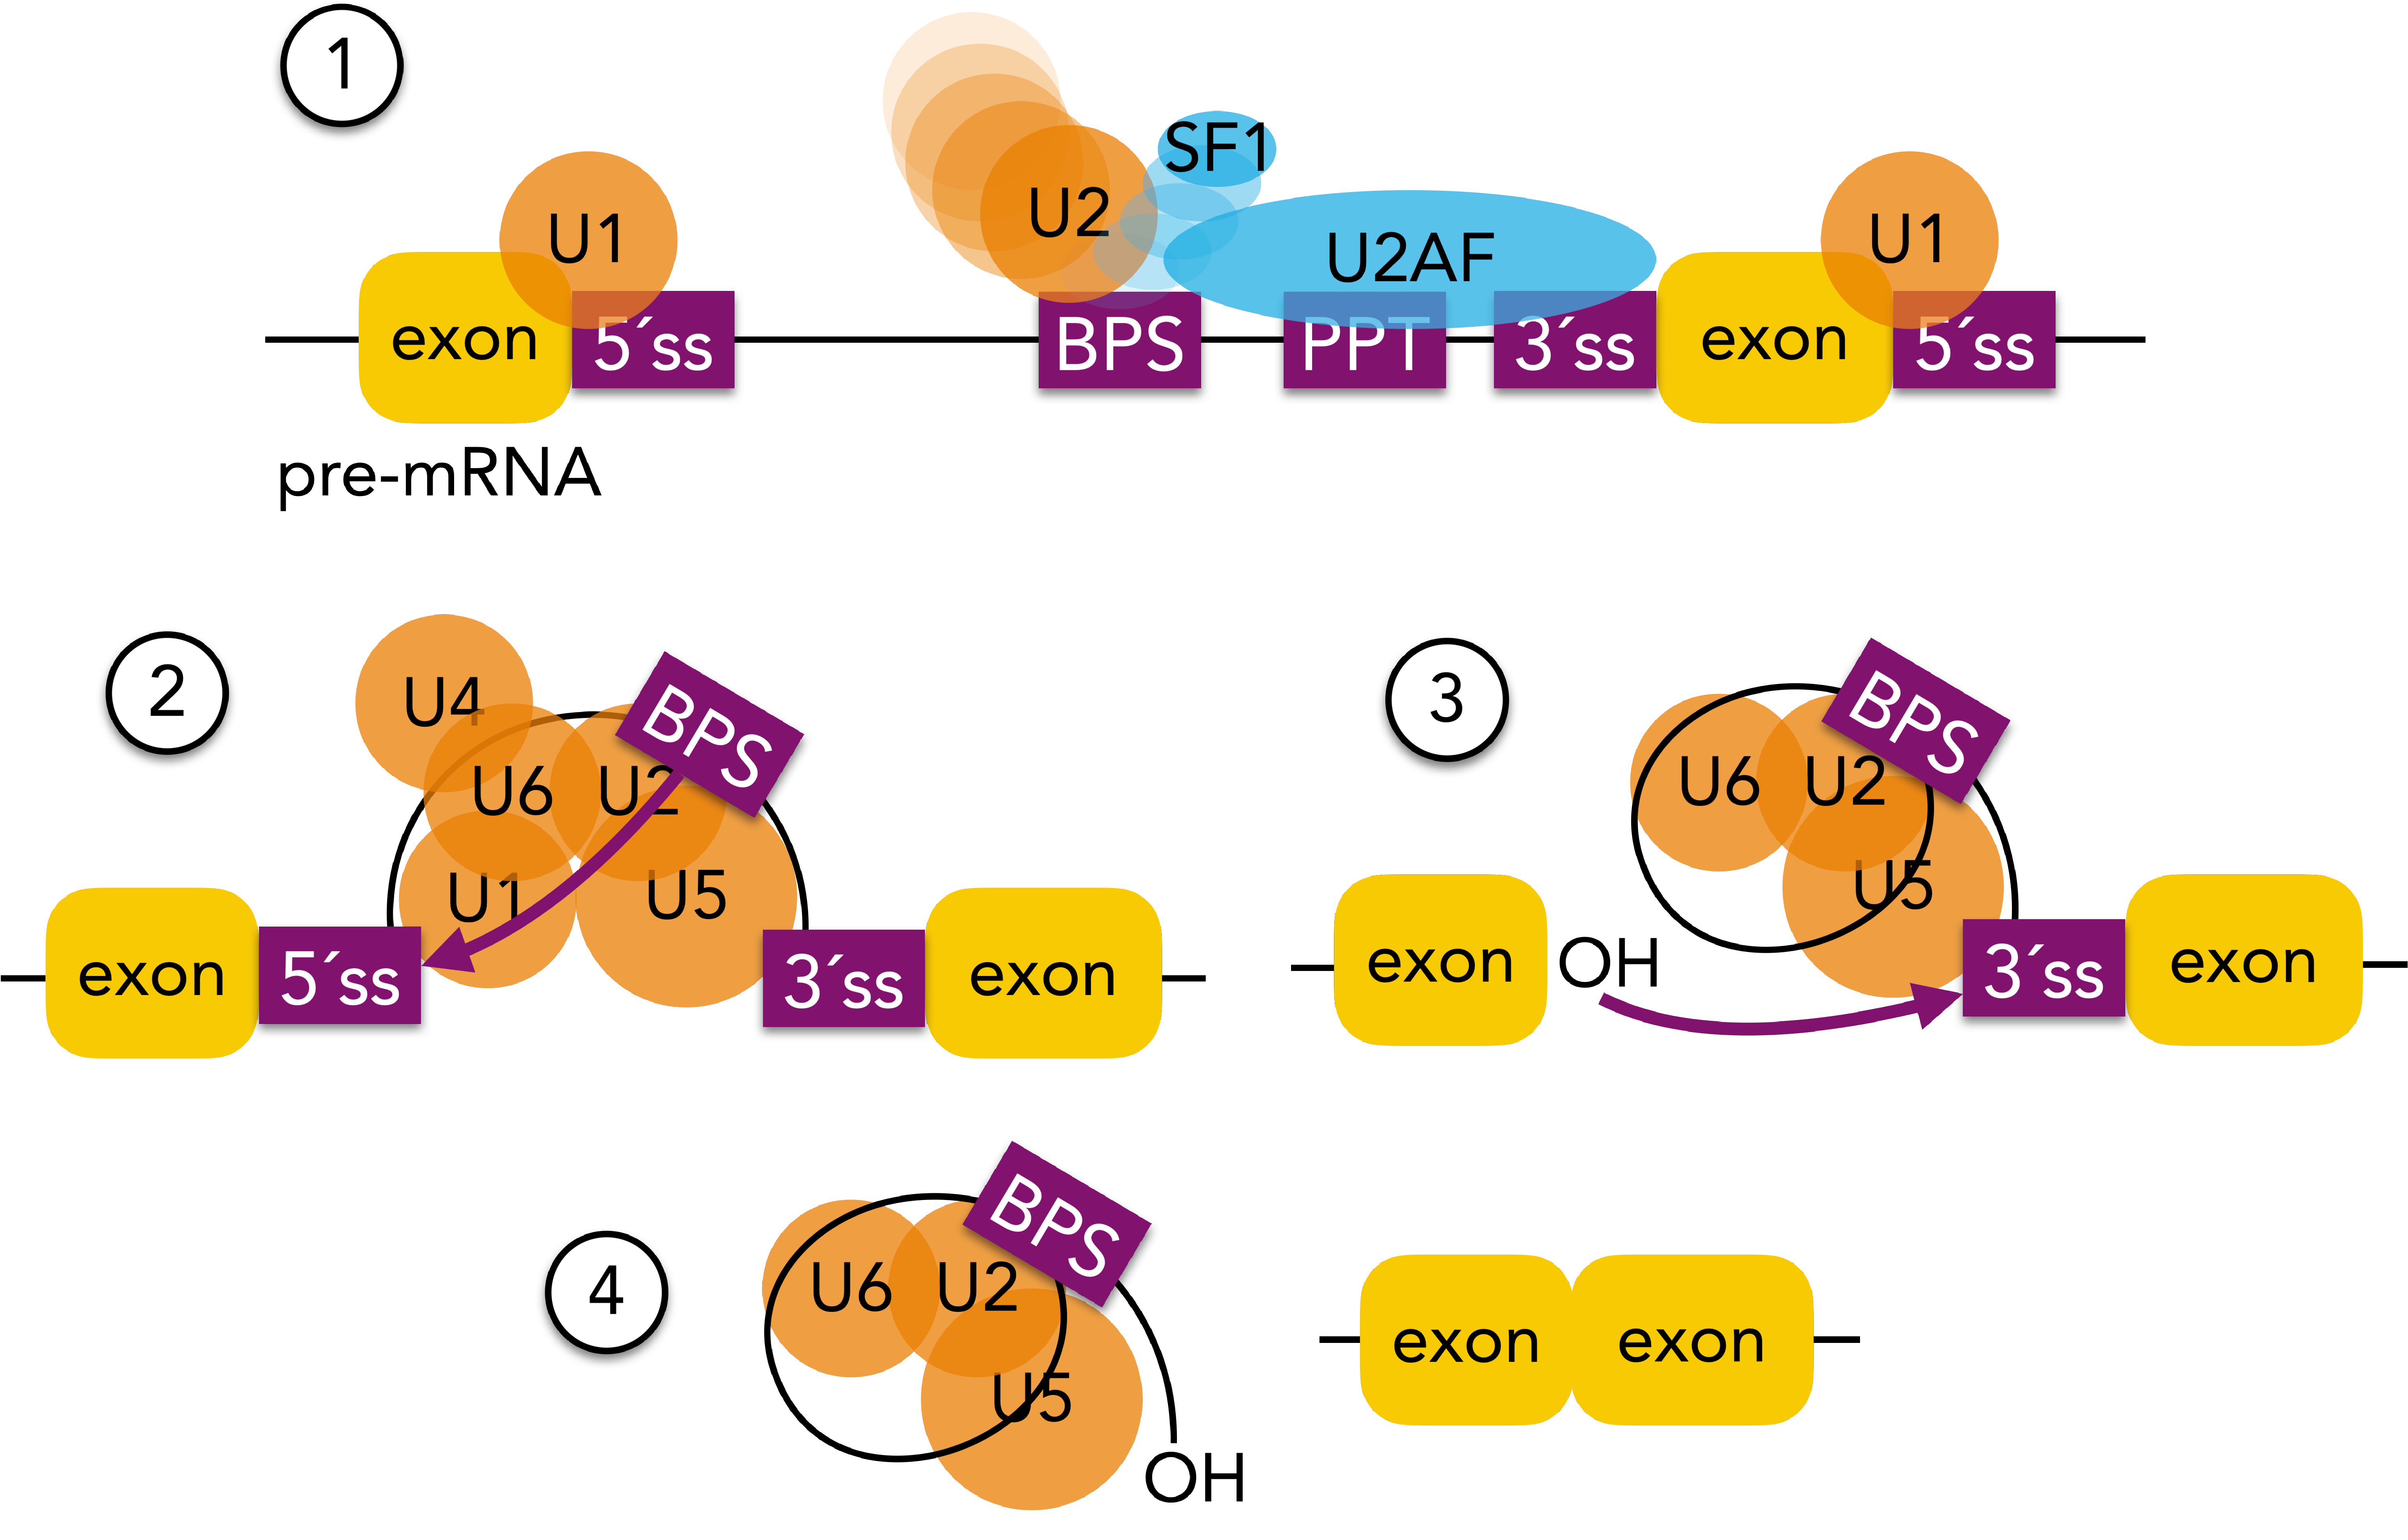
\includegraphics[width=.5\linewidth]{images/intro/spliceosome-assembly}
  \caption[Spliceosome assembly and splicing reactions]{\textbf{Spliceosome assembly and splicing reactions.} (1) U1 snRNP binds to the 5$'$ splice site (5$'$ss), whereas the splicing factor 1 (SF1) and U2AF proteins bind to the branch point site (BPS), the polypyrimidine tract (PPT), and 3$'$ splice site (3$'$ss). The interaction between U1 and U2 snRNPs results in the formation of the pre-spliceosome. (2) The first splicing reaction is performed after the recruitment of the U4/5/6 snRNPs through a nucleophilic attack from the adenosine in the BPS to the 5$'$ss of the upstream exon. (3) The intron lariat is then formed. The free 3$'$ hydroxyl group performs a nucleophilic attack to the phosphate of the 3$'$ splice site of the downstream exon. (4) Finally, the intron lariat is released and both exons are ligated.}
\end{figure}

However, not all introns require the presence of the spliceosome to be spliced out. During the 1980s, Thomas Cech identified rRNAs that underwent self-splicing by breaking and forming covalent bonds with no associated proteins \cite{kruger:1982wk}, whereas Sidney Altman identified that the RNA subunit of a complex of proteins and RNAs (ribonulceoprotein complex) was essential for tRNA splicing and was able to cleave tRNAs \emph{in the total absence of proteins} \cite{altman:1986wp}. These RNAs with enzyme-like proteins were named ribozymes and they may have been a paramount mechanism that conferred evolutionary flexibility in life forms of yore, one of the pillars that originated the RNA world hypothesis \cite{kruger:1982wk,gilbert:1986td}. From fungi to plants and vertebrates, many spliced genes across eukaryotic organisms share consensus sequences at their branch point, as well as their 5$'$ and 3$'$ splice sites, potentially making splicing one of the first molecular catalysts that appeared in living beings \cite{sharp:1985th}. Primary transcripts from yeast can be spliced with the mammalian splicing machinery \cite{sharp:1985th}.
% conservation of AS across tissues and organisms (Barbosa-Morais et al.)

By 1989, it was known that alternative splicing is differentially regulated across cell types, development stages and tissues in eukaryotes, i.e. the same gene can lead to different, context-dependent spliced transcripts \cite{smith:1989tr}. This regulation occurs via the interplay between trans-acting factors -- RNA-binding proteins (RBPs) -- and the cis-acting sequence elements to which they bind to, promoting or repressing the inclusion of alternative sequences \cite{smith:1989tr}. Multiple types of alternative splicing have also been described, including skipped exons, mutually exclusive exons, alternative 5$'$ and 3$'$ splice sites, alternative first and last exon and intron retention \cite{smith:1989tr}.
% add figure + cite newer review on splicing

% 1989-1996: minor spliceosome splices less than 1\% of all human introns

% By the early1990s, the spliceosome was shown to be assembled at each splice event and to act in a dynamic stepwise process that links exons in mRNAs (for review, see Wahl et al. 2009).

Among other molecular mechanisms, alternative splicing made clear that an organism complexity is not limited to the genome size or the number of protein-coding genes \cite{}. After all, the Australian lungfish (\emph{Neoceratodus forsteri}) is the animal with the largest genome size (44 000 million base pairs), 14 times larger than that of humans (3 000 million base pairs) and 244 times larger than the fruit fly \emph{Drosophila melanogaster} (180 million base pairs) \cite{meyer:2021vn,dmelanogaster}. And yet, their genomes harbour 31 000, 20 000 and 14 000 protein-coding genes, respectively, numbers in the same order of magnitude, whereas the remaining genome of these species are composed of intergenic regions and introns with high repeat content \cite{meyer:2021vn,dmelanogaster}. Notably, the fruit fly has 38 000 alternative transcripts generated from a single gene (Dscam) \cite{schmucker:2000wf}. The multiple isoforms of this gene play a role the immune system of the fruit fly and may lead to more antigen diversity, thus increasing the evolutionary flexibility of the fruit fly.
% how many functional proteins? what more about this example? maybe useful to talk about other topic such as trans/cis-acting elements or spliceosome?

% 90-95\% of human genes are spliced
% variation of AS across tissues

% Coupling of Transcription and Splicing?

Alternative splicing is deregulated in multiple disease contexts, including cancer, neurodegeneration and muscular dystrophies \cite{gallego-paez:2017wc,montes:2019ww}. For instance, changes in splicing factors and subsequent  perturbations to splicing can affect multiple hallmarks of cancer \cite{zhang:2021wn}. Therefore, multiple potential splicing-targeting therapies have been developed based on antisense oligonucleotides, small molecules and novel techniques \cite{montes:2019ww}.
% Discuss disease-related NMD?
% Alternative splicing in ncRNAs?

% AS during organ development: https://www.nature.com/articles/s41588-021-00851-w

% Around 1980, Michael Smith developed a method by which combined DNA building blocks could be artificially bonded with DNA molecules that were then inserted into an organism where they were copied. The result was an artificial mutation; the genome was altered so that specific amino acids in the proteins were replaced. The opportunities this method provides to tailor proteins have been of major importance in both research and industry.
% In 1989, through studies of bacterial viruses, Paul Modrich showed how methyl groups attached to the DNA molecule act as signals for repairing incorrect replications of DNA. These discoveries have increased our understanding of how the living cell works, the causes of cancer and about aging processes.
% 1998: RNAi -- gene silencing discovered by Andrew Fire and Craig Mello

\section{Bioinformatics}

% The fact that we need to specifically name the computer-aided analysis as sub-field of biological research demonstrates how bioinformatics is not as widely used as it should.

% 1. sequencing, annotation and comparison
% 2. comparative sequence analysis
% 3. expression analysis
% 4. structure prediction
% 5. network modelling

Bioinformatics is a multidisciplinary field based on the usage and development of computer programs to analyse large-scale biological data \cite{gauthier:2018ws}. The first bioinformatic analyses were performed on proteins. Following Sanger's work in 1959 on identifying the amino-acid composition of the protein insulin in multiple species, many proteins started being sequenced \cite{sanger:1955uw,ryle:1955wf,harris:1956ut,gauthier:2018ws}.
% He used acids to break the molecule into smaller parts, which were separated from one another with the help of electrophoresis and chromatography. Further analyses determined the amino acid sequences in the molecule's two chains, and in 1955 Frederick Sanger identified how the chains are linked together.
Pointing to such studies, Crick predicted in 1958 that:

\begin{displayquote}[\cite{crick:1958ws}]
Biologists should realize that before long we shall have a subject which might be called 'protein taxonomy' - the study of the amino acid sequences of the proteins of an organism and the comparison of them between species.
\end{displayquote}

For that to come to fruition, more distinct proteins from different species would first need to be fully sequenced for comparison. A technique known as Edman degradation was popularly used at the time to sequence proteins: the amino acids were identified by chemically fragmenting the protein, identifying the first 50-60 amino acids of each fragment. Afterwards, the full protein sequence is reconstructed based on its overlapping fragments, a long and tedious process performed by hand \cite{gauthier:2018ws,edman:1949ww}. All these limitations meant that only 6 different proteins were fully sequenced by 1962 \cite{dayhoff:1962up}. To overcome those difficulties in the reconstruction step, Margaret Dayhoff and Robert Ledley developed COMPROTEIN, the first bioinformatics program \cite{gauthier:2018ws,dayhoff:1962up}. COMPROTEIN allows to compare a high number of small peptide fragments and suggests possible full protein sequences \cite{dayhoff:1962up}. By 1965, the number of published protein sequences grew up to 65 and were published by Dayhoff in the first protein database, otherwise known as the book entitled \emph{Atlas of Protein Sequence and Structure}\cite{dayhoff:1965vv}.

In 1963, Linus Pauling and Emile Zuckerkandl discussed that cross-species comparative analysis of protein sequences could help determine the original protein sequence of their common ancestor and measure the evolutionary distance of the sequence of each species to that of their common ancestor \cite{pauling:1963uo}. However, these protein comparison methods were performed by hand, which meant that they were only practical for closely-related proteins such as homologs from different mammals \cite{gauthier:2018ws}. Since 1970, computer-assisted phylogenetics started being a reality with the introduction of the Needleman-Wunsch algorithm \cite{needleman:1970vq} and variants, such as the Smith-Waterman algorithm \cite{smith:1981up}. These programs computationally measure the distance between two sequences by pair-wise comparison of amino acids between protein sequences \cite{needleman:1970vq,smith:1981up}.

% Substitution matrices in 1978:
% - Dayhoff, M.O., Schwartz, R.M., Orcutt, B.C. (1978) "A model of evolutionary change in proteins." In "Atlas of Protein Sequence and Structure, vol. 5, suppl. 3," M.O. Dayhoff (ed.), pp. 345-352, Natl. Biomed. Res. Found., Washington, DC.
% - Schwartz, R.M., Dayhoff, M.O. (1978) "Matrices for detecting distant relationships." In "Atlas of Protein Sequence and Structure, vol. 5, suppl. 3," M.O. Dayhoff (ed.), pp. 353-358, Natl. Biomed. Res. Found., Washington, DC.

% conservation, structural conformation, functional domains

% when did computers started being used?

Years after automatic protein sequencing machines being available based on Edman degradation -- \emph{protein sequenators} as first called in 1967 \cite{edman:1967tc} --, DNA sequencing methods were presented based on electrophoresis: the enzymatic Sanger method (also known as dideoxy method) \cite{sanger:1977vp} and the chemical degradation method Maxam-Gilbert sequencing \cite{maxam:1977vy}. These tedious and slow processes required manual intervention \emph{at both the experimental and interpretative levels} \cite{hood:1987va}.

Leroy Hood and Lloyd Smith published a 1987 report on an instrument to automate the experimental procedure based on the Sanger method followed by computer analysis to determine the sequence of DNA fragments (i.e. base calling): the Applied Biosystems DNA sequencer, the first commercialised automated machine to sequence DNA \cite{hood:1987va}. Their article also discusses experimental issues with sequencing repetitive DNA regions, storing and sharing the big amount of data produced in the following years in \emph{data banks}, as well as the algorithms required to quickly retrieve sequence from those databases -- obstacles that impaired large-scale DNA sequencing, specially of the whole human genome \cite{hood:1987va}.

Later, the advent of Next-Generation Sequencers (NGS) allowed the massive parallel sequencing of nucleic acids. These techniques use alternative methods to Sanger sequencing to efficiently sequence DNA or RNA fragments simultaneously.

As the techniques to retrieve biological data were optimised, more and more data started being generated and published in public databases such as the Protein Data Bank \cite{protein-data-bank:1971tm} and GenBank \cite{burks:1985ts}. Computers were no longer optional to survive the tsunami of biological data and new popular bioinformatic algorithms started to emerge. More advanced sequence aligners, such as CLUSTAL in 1988, efficiently allowed to align multiple sequences of amino acids or nucleotides from pairwise sequences \cite{higgins:1988ul}. In 1990, BLAST was presented as an efficient algorithm to quickly compare a DNA or protein sequence against the ever-increasing number of molecular sequences from biological databases \cite{altschul:1990vt}.

In 1995, the first complete sequence of a free-living organism was published for the bacterium \emph{H. influenzae} \cite{fleischmann:1995vz}. From 1996 to 2000, the whole genomes of multiple other organisms were sequenced, including for the yeast \emph{S. cerevisiae} \cite{goffeau:1996tk}, the nematode \emph{C. elegans} \cite{the-c.-elegans-sequencing-consortium:1998wf}, the fruit fly \emph{D. melanogaster} \cite{myers:2000wk,adams:2000tj}, and the plant \emph{A. thaliana} \cite{the-arabidopsis-genome-initiative:2000tm}. In 2004, the Human Genome project was considered finished with its goal of publishing the human genome to the scientific community, leaving 8\% to be determined due to technical limitations \cite{consortium:2004wi,nurk:2021up}. Many advantages come from sequencing whole genomes, specially the \emph{near complete} human genome:

\begin{displayquote}[\cite{consortium:2004wi}]
It allows systematic searches for the causes of disease -- for example, to find all key heritable factors predisposing to diabetes or somatic mutations underlying breast cancer -- with confidence that little can escape detection. It facilitates experimental tools to recognize cellular components -- for example, detectors for mRNAs based on specific oligonucleotide probes or mass-spectrometric identification of proteins based on specific peptide sequences -- with confidence that these features provide a unique signature. It allows sophisticated computational analyses -- for example, to study genome structure and evolution -- with confidence that subtle results will not be swamped or swayed by noisy data. At a practical level, it eliminates tedious confirmatory work by researchers, who can now rely on highly accurate information. At a conceptual level, the near-complete picture makes it reasonable for the first time to contemplate systems approaches to cellular circuitry, without fear that major components are missing.
\end{displayquote}

% Third-generation sequencing: longer reads
More recently, the Telomere-to-Telomere (T2T) consortium exploited current long-read sequencing (third-generation sequencing), along with other sequencing technologies, in order to fully unravel the gapless assembly of the human genome for use in biomedical research \cite{nurk:2021up} \footnote{Although the most recent T2T pre-print manuscript from 2021 describes ongoing work for the missing chromosome Y \cite{nurk:2021up}, the latest assembly published in 24 January 2022 (CHM13 T2T v2.0) includes the full human genome sequencing: \alink{ncbi.nlm.nih.gov/assembly/GCA_009914755.4}.}.

\subsection{Transcriptomics}

The term \emph{omics} encompasses all fields in life sciences that analyse large-scale data to better understand the molecular world \cite{yadav:2007uy}. The first word using the \emph{-omics} suffix dates back to a 1986 conference meeting among peers and beers. While discussing the name for a new journal intended to include sequencing data, gene mapping and new genetic technologies, Thomas Roderick proposed a name to illustrate a \emph{new way of thinking about biology}: genomics \cite{yadav:2007uy,kuska:1998ta}. The genomics field is concerned with the study and cross-species comparison of genomes \cite{kuska:1998ta}.

In the same vein, transcriptomics is the field that studies the transcriptome: the set of RNA transcripts\footnote{Depending on the context, the term \emph{transcriptome} may exclusively refer to the study of mRNA transcripts instead of all RNA transcripts.}, as first defined in 1996 \cite{pietu:1999tl}. Transcriptomics is usually performed based on data generated from high-throughput technologies that allow to simultaneously analyse the expression of multiple RNAs. Diverse technologies have been proposed for the large-scale study of transcripts since the 1990s, including:

\begin{itemize}
	\item \textbf{Expressed Sequence Tags (EST)}: proposed in 1991 as a pilot experiment to focus on the expressed genes via the Human Genome project \cite{adams:1991ua}. EST allows to identify random sequences of complementary DNA (cDNA), i.e. reverse transcribed mRNA sequences.%\footnote{The article starts with an interesting motivation: \emph{The Human Genome is estimated to consist of 50 000 to 100 000 genes, up to 30 000 of which may be expressed in the brain.} \cite{adams:1991ua}. The number of genes is still debated nowadays, but a recent pre-print estimates them to be around 43 162 genes, of which 21 306 are protein-coding genes \cite{pertea:2018ty}.}
	\item \textbf{Serial Analysis of Gene Expression (SAGE)}: developed in 1995 for the \emph{quantitative and simultaneous analysis of a large number of transcripts}. \cite{velculescu:1995vx}
	\item \textbf{Microarrays}: first mentioned in a 1995 study as a method to measure simultaneously the expression of multiple genes in an high-density array with small wells via cDNA hybridisation \cite{schena:1995tu}. According to the article: \emph{The large and expanding database of complementary DNA (cDNA) sequences from many organisms presents the opportunity of defining these patterns at the level of the whole genome} \cite{schena:1995tu}. The first genome-wide microarray study was later conducted in yeast during 1997 \cite{lashkari:1997wh}, followed by the whole human transcriptome using infant human brains in 1999 \cite{pietu:1999tl}.
	\item \textbf{Short-read RNA sequencing (RNA-seq)}: first mentioned in 2008 as a novel quantitative technique based on the Illumina platform to sequence cDNA fragments in a massively parallel method \cite{nagalakshmi:2008vs}. This method is followed by computational mapping of resulting short reads (spanning 50 base pairs at the time, currently along the lines of 150-200 base pairs) to a genome of reference, allowing to unravel the transcriptional regions of the yeast. More accurate and sensitive than microarray methods, RNA-seq can quantify more lowly-expressed transcripts than microarrays by avoiding cross-hybridisation issues. RNA-seq data also allows to accurately identify exon boundaries and therefore introns, crucial for alternative splicing analysis \cite{nagalakshmi:2008vs}.
	\item \textbf{Long-read RNA-seq}: RNA-seq methods that generate reads over 1000 base pairs and up to 10000 base pairs, allowing to sequence full transcripts in some cases.
	\item \textbf{Direct RNA-seq}: direct sequencing of RNA molecules without modification or reverse transcription.
%	\item \textbf{Single-cell RNA-seq (scRNA-seq)}: reported in 2009, 
%	\item \textbf{Ribosome profiling}:
%	\item \textbf{Spatial RNA-seq}:
%	\item \textbf{Nascent RNA sequencing}: 
\end{itemize}

Currently, short-read RNA-seq is the most commonly used approach for its relative cost and accuracy.

% paired-end vs single-end?
\subsubsection{RNA-seq data analysis}

Before transcriptomic analyses, transcripts are isolated by first disrupting cell membranes and neutralising RNA-degrading enzymes (RNases). As over 90\% of the extracted RNA is ribosomal, depletion of rRNAs and/or enrichment of the desired species are required for proper analysis. Most datasets currently enrich for polyadenylated RNAs (i.e. isolating mostly mature mRNAs).

\begin{figure}[!hb]
  \centering
  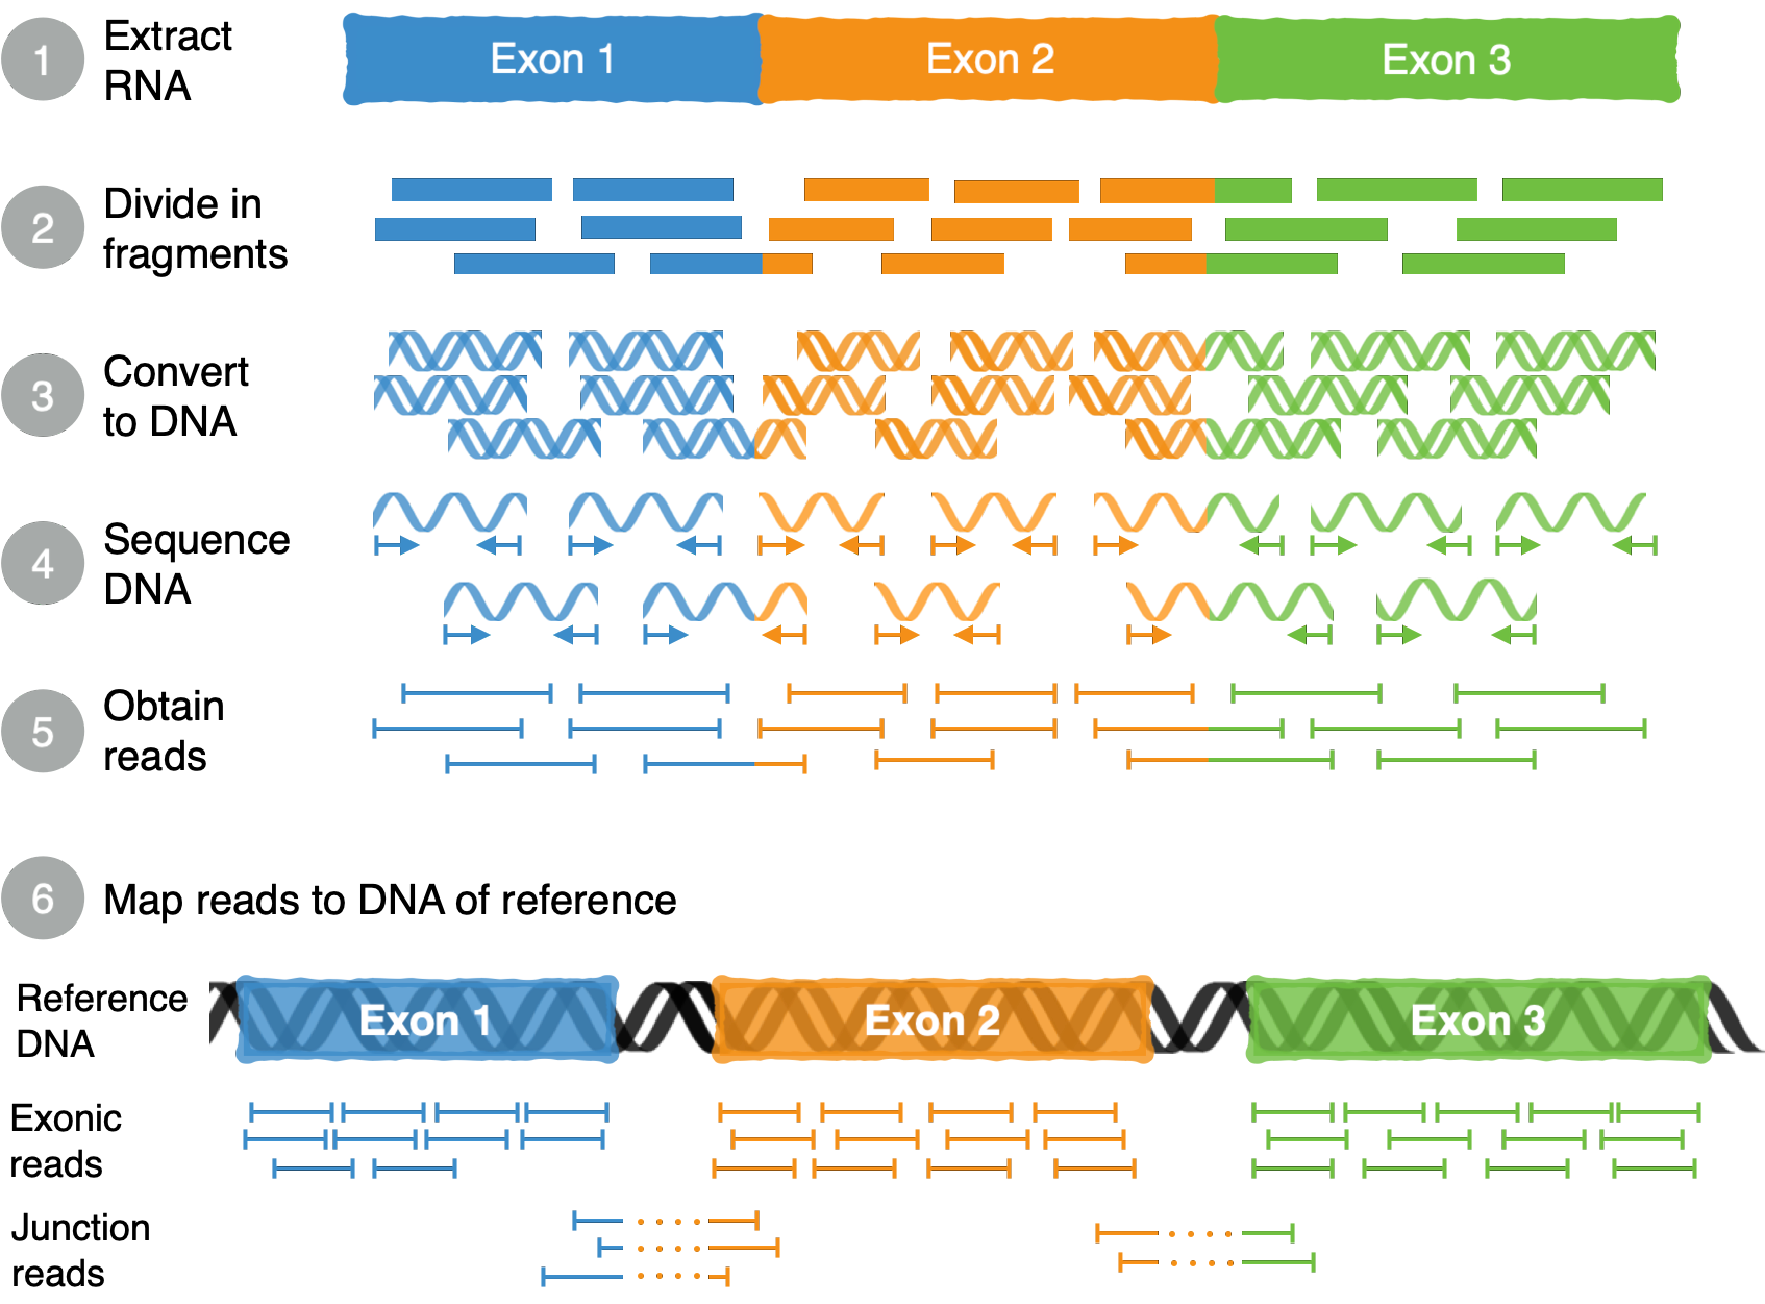
\includegraphics[width=1\linewidth]{images/intro/rna-seq}
  \caption[RNA sequencing and read mapping]{\textbf{RNA sequencing and read mapping.} RNA is first extracted from a sample (1) and divided into small fragments (2). These fragments are then converted to DNA (3) and sequenced, producing short text strings called reads (4). Finally, these reads are mapped to a DNA of reference (5) allowing to reconstruct the extracted mRNA and identify exon coordinates in the reference DNA.}
  \label{fig:RNAseq}
\end{figure}

% https://pubmed.ncbi.nlm.nih.gov/26813401/
% experimental design: rRNA-, library type, sequencing length, replicates, sequencing depth

After extraction, transcripts are sequenced. RNA-seq is a standard practice to better understand what features (genes, transcripts, exons, etc.) were expressed in the moment of RNA extraction, like taking a snapshot of a sample to later analyse it. Before the snapshot, the whole family of transcripts is prepared to look good in the photo: RNAs are fragmented in multiple sequences and converted to cDNA via reverse transcription enzymes. Finally, cDNA is sequenced in order to obtain reads, computer strings of nucleotides of the fragmented RNA sequences.
% Oxford Nanopore allows for direct RNA sequencing.

The number of sequencing reads per sample (known as sequencing depth or library size) depends on the intent of the experiment. The quantification of lowly expressed genes, for instance, requires a larger number of reads compared to highly-expressed genes, in order to detect more gene and with higher precision. To assess the sequencing depth required for a certain experiment, we can look at saturation curves.

Using 3 or more technical replicates allows to reduce external variability. Technical biases may occur, specially when performing multiple batches, as usually done for big sample sizes. To minimise such biases, it is important to use proper controls, randomise sample processing and manage sequencing reads. It is also possible to use batch-correction algorithms, such as ComBat \cite{johnson:2006tj,zhang:2020uq}.

Quality control is a major step in RNA-seq data analysis. Low quality reads, duplicated sequences and overrepresented \emph{k}-mers are some metrics used by FastQC to identify issues with reads from a particular sample that may be resolved by trimming reads or even discarding samples \cite{andrews:2019vg}. % When performing clustering analyses (after data normalisation), it is expected that reads from replicates cluster together, unless there are potential batch effects or technical biases.

To reconstruct the moment at which the RNA was sequenced, fragmented reads are compared against a reference genome or transcriptome\footnote{Alternatively, the transcriptome may be reconstructed \emph{de novo} from available transcripts, as usually employed for organisms without any available reference. Given that short reads may be insufficient for this operation, newer technologies based on longer reads are preferentially used.}, allowing to understand where the sequences most likely come from and which features (genes, transcripts, exons, etc.) are more expressed. Unfortunately, some of those sequences fit in multiple places, such as reads from repetitive regions and so are distributed based on empiric evidence and/or randomness. Shorter reads are more prone to multi-mapping (less chances of sequencing unique regions) and their alignment may prove ambiguous. Such issues can be mitigated by using paired-end reads and higher read coverage.

% pre-processing (low count removal, technical bias, normalisation)
Based on the number of reads that were aligned on each region of the genome or transcriptome, it is possible to quantify features of interest, e.g. estimate gene, transcript or exon expression. To make these counts comparable across samples, they are normalised by transcript length, number of total reads and/or sequencing biases. Afterwards, gene expression can be linearly modelled across multiple conditions to identify differentially expressed genes \cite{conesa:2016vw}.

Specifically, the study of alternative splicing has been greatly enhanced with the advent of cheaper, high-throughput technologies, since higher read coverage greatly benefits alternative splicing analysis \cite{}. % why?
One approach to study alternative splicing changes is based on the differential expression of isoforms of a single gene (e.g. CuffDiff2 \cite{trapnell:2013uv}). However, isoform expression estimation based on short reads can be inaccurate. % why?
Other methods based on exon and junction reads specifically identify alterations in events of alternative splicing \cite{conesa:2016vw}: comparing the expression of different exons (differential exon usage, e.g. DEXseq \cite{li:2015tn}), estimating the percentage of alternative sequence inclusion (percent spliced-in, e.g. VAST-TOOLS \cite{irimia:2014wt,tapial:2017ui} and rMATS \cite{shen:2014tk}) or based on graph theory to identify alternative splicing modules (e.g. DiffSplice \cite{hu:2012uw}).
% differential splicing in RNA-Seq data: https://humgenomics.biomedcentral.com/articles/10.1186/1479-7364-8-3

% functional profiling (GSEA, pathway analyses)
% quantification measures
% ncRNAs, long reads, scRNA-seq

% pre-processing (low count removal, technical bias, normalisation)
Transcriptomic studies like those performed using RNA-seq data allow to identify altered phenotypes across development stages and pathological subtypes (such as stages of a disease progression), explore the molecular mechanisms underlying a phenotype and pinpoint disease biomarkers. These type of studies can be enhanced by integrating multiple data, such as genetic variants, methylation, proteomics and other omics data \cite{chang:2013ww,perez-riverol:2019uk}.

\subsection{Publicly-available big data}

The development and economic feasibility of next-generation RNA sequencing lead to a wealth of publicly-available sequencing data that can be integrated with available clinical, drug-associated, mutation annotation, methylation and proteomic data. The public availability of these datasets to the research community ensures not only more transparency and reproducibility, but also bigger opportunities to unravel molecular mechanisms, identify more accurate biomarkers and predict novel treatments without spending fortunes in grants to repeat experiments already performed by others, enabling new advances in personalised medicine via data sharing \cite{rockhold:2019ws}. It also means that data can be exploited for other purposes other than those initially intended.

However, the ever-increasing amounts of large-scale data -- \emph{big data} -- require more and more computational resources for their processing and analysis \cite{gauthier:2018ws}, specially when used to train machine learning models. These analyses can be quite prohibitive for non-specialised researches interested in quick biological queries. To satisfy such needs, some projects provide open access to pre-processed data via download (e.g. sequence aligned and normalised data) and apps for data exploration:

\begin{itemize}
	\item \textbf{The Cancer Genome Atlas (TCGA)} with molecular and clinical data for more than 30 cancer types (e.g. breast cancer and glioma) from more than 10 000 human samples \cite{chang:2013ww}. Multiple web apps tap into the data from this behemoth, including TCGASpliceSeq \cite{ryan:2016tm} and Xena Browser \cite{goldman:2020ub}.
	\item \textbf{The Genotype Tissue Expression (GTEx)} project, a repository of gene expression data for more than 40 tissues, totalling more than 15 000 human samples \cite{lonsdale:2013uo}. GTEx Portal (\alink{gtexportal.org}) allows to inspect, for instance, the expression values of specific genes and isoforms across multiple tissues.
	\item The \textbf{recount} project has processed RNA-seq data from Sequencing Read Archive (SRA) \cite{collado-torres:2017uw,wilks:2021uc}.
\end{itemize}

Even with the increasing economic feasibility of RNA-seq, cheaper technologies allow measuring gene expression for larger sample sizes, like in the case of L1000, an inexpensive assay platform where the profiling of 978 transcripts allows to estimate the expression of around 12000 genes via computational inference \cite{subramanian:2017ul}. The development of L1000 was crucial to establish the Connectivity Map (CMap), a collection of almost half a million gene expression signatures derived from chemical and genetic perturbations across multiple cell lines, dosages and timepoints \cite{subramanian:2017ul}. CMap data has been used in multiple contexts, including to identify inhibitors of the stemness signature in multiple TCGA cancer types \cite{malta:2018uj}, to train machine learning models for designing molecules inducing desired transcriptomic changes \cite{mendez-lucio:2020th} and to predict clinically-approved drugs for repurposing as SARS-CoV-2 antiviral agents \cite{le:2021uq}.

To find effective novel treatments, it is important to understand how different cell respond to specific compounds. Multiple drug sensitivity datasets contain compound toxicity data across diverse cell lines, including the NCI-60 \cite{shoemaker:2006wi}, the Cancer Therapeutics Response Portal (CTRP) \cite{seashore-ludlow:2015ws} and the Genomics of Drug Sensitivity in Cancer (GDSC) \cite{yang:2012vk}. Alongside gene expression data for each cell line, these datasets integrate data that allows to, for instance, pinpoint drugs that selectively target malignant cells.
% examples of works made possible thanks to these datasets

Although the number of datasets is getting larger every day, many obstacles render data inaccessible, including lack of standardised formats for storing molecular data, difficulty in retrieving human raw data, and inefficient communication between different platforms \cite{rockhold:2019ws}. Another major hurdle of data dissemination is privacy issues and insufficient anonymisation of clinical data sharing, that can scare away individuals from sharing their personal data in public platforms.

Together with open data, there has also been a push for open access to scientific articles, an important step in disseminating science to everyone, including non-scientists. The publication of pre-prints has also been increasing, allowing for faster research dissemination and for early feedback from peers.

Open source is also important to easily allow reproducing published data analysis. Still, code alone may not suffice and the environment changes (e.g. different software versions and operative systems) may lead to unexpected results. To overcome those difficulties, standard tools can be used like Nextflow to run scalable computational pipelines that may employ Docker containers for reproducibility in different machines \cite{di-tommaso:2017vq}.

\subsection{Software development}

% The evolution of software + hardware?
The nature of software has changed throughout the years from simple instructions that calculate Bernoulli numbers, the first published computer program by Ada Lovelace in 1843, to the "foundation for ultra-reliable software design", the on-board flight system that assisted the first moon landing with a crewed mission in 1969, supervised by Margaret Hamilton.

Software plays an important role in society nowadays and scientific research is no exception. For instance, the analysis of RNA-seq data requires specialised tools for quality control, sequence alignment, feature quantification, statistical analyses and visualisation techniques to assist researchers and clinicians in the biological interpretation of their results \cite{conesa:2016vw}. However, many of these specialised tools are developed by scientists with little programming knowledge and may lead to software with structural  issues, e.g. non-user-friendly interfaces, unreproducible results, poorly documented systems, and reliance on deprecated technologies \cite{storer:2017tr,silva:2017wl}.

% Design thinking

To mitigate such issues, scientific software developers can adopt iterative approaches (like agile methodology) that fits the ever-evolving nature of scientific software development. Iterative development facilitates incremental improvement and delivery of stable software iterations by continuously planning and performing small tasks that are evaluated and prioritised based on the project context \cite{storer:2017tr,silva:2017wl,dyba:2009tc}. These development approaches go through a continuous cycle of several steps, including:

\begin{itemize}
    \item{\textbf{Requirement analysis} where we identify stakeholders and their requirements of what the system should do (functional) and that should characterise the system (non-functional; e.g. modular, reliable, secure, easy-to-use and scalable) \cite{silva:2017wl,hewitt:2019uj}. The initial requirements of a system tend to (and should) be of higher-level, but increase in complexity as the project advances: in simpler terms, a first version of the software should be simple and improved upon to get more features over time \cite{silva:2017wl,kanat-alexander:2012ve}.}
    \item{\textbf{Design} concerns with the technologies to use during software development (e.g. frameworks for web app development and cloud hosting solutions for distribution), as well as the proper implementation of new features in the current software iteration or the integration with other programs via standard application programming interfaces (APIs), for instance. Good software design should allow to extend current functionality with as few changes to the core of the program as possible.}
	\item{\textbf{Development}, such as code structuring, feature implementation, bug fixing and code optimisation.}
	\begin{itemize}
	    \item Version control systems (e.g. git) track changes to files in a project, allows to easily integrate code from different developers and compare files across diffterent versions \cite{silva:2017wl,ford:2021ub}.
		\item Kanban-like boards allow to visualise and manage the project workflow, where features and bugs can be commented on and tracked \cite{silva:2017wl,hewitt:2019uj}.
		\item Comprehensive documentation (tutorials, manuals, wikis, inline source code comments, etc.) is crucial to showcase the program and explain how features work via functions' description and examples to end-users and developers alike and can be written in plain text, Markdown and other common file formats \cite{storer:2017tr,silva:2017wl,kanat-alexander:2012ve,ford:2021ub}. For development purposes, good documentation facilitates the maintenance and reusability of the program. Multiple tools automatically generate documentation from inline source code comments for different programming languages that can be automated, including roxygen2 for R \cite{wickham:2021wt} and Sphinx for Python \cite{silva:2017wl,hewitt:2019uj}.
	\end{itemize}
	\item{\textbf{Testing} via unit tests, usability tests, performance tests, integration tests and security tests. Testing should be performed in multiple environments (e.g. different versions of programming languages, dependencies, operating systems and web browsers) \cite{silva:2017wl,kanat-alexander:2012ve,ford:2021ub}. The portion of the code covered by unit tests (written to check particular parts of code return the expected output when run) can be evaluated using code coverage tools such as CodeCov, allowing to understand how much of the code is being tested \cite{hewitt:2019uj}.}
	\item \textbf{Software distribution (deployment)} is related with the release of program iterations to the hands of end-users: the easier it is to deploy, the faster new iterations can be released with new features and bug fixes \cite{ford:2021ub}.
	\begin{itemize}
		\item Software can be distributed as web-browser-based applications (web apps) or desktop apps. Containerisation (e.g. via Docker) also helps distributing complex software and its dependencies in an easier way. There are also many available repositories that allow to store code and/or compiled programs (GitHub to store git projects, DockerHub for Docker images, Bioconductor for bioinformatic R packages \cite{huber:2015wt} and CRAN for generic R packages).
		\item When distributing code and/or programs, licensing must be defined since the first general release to avoid code misuse by third parties \cite{silva:2017wl}. Different types of licenses can be chosen, allowing to decide whether the program can be modified, redistributed, used for commercial purposes and whether there are special conditions (e.g. any code derivation must be open-source and modifications must retain same license) \cite{silva:2017wl}.
		\item User feedback via bug reports and feature requests should be collected and considered for future  iterations.
	\end{itemize}
\end{itemize}

To facilitate continuous iterations, some steps can be automated using continuous integration (CI) tools, allowing to compile, run, test, deploy and document software. Those steps can then run in a multitude of environments whenever new changes are integrated in the code or at a regular interval (e.g. weekly) to ensure compatibility of the same software version with newer versions of external dependencies. Automation tools are crucial to quickly detect issues in a multitude of reproducible contexts and to promote code quality, testability, integration and continuous feedback \cite{silva:2017wl,hewitt:2019uj,ford:2021ub,storer:2017tr}.

Many popular CI tools, like Travis-CI, GitHub Actions and AppVeyor, can be used for free in open-source projects. This approach promotes software quality by allowing peer-reviewing the code, reusing parts, fixing bugs, extending features and collaborating with external developers \cite{silva:2017wl,hewitt:2019uj}, as well as it facilitates analysis transparency and reproducibility \cite{silva:2017wl}. Moreover, it has educational value, allowing others to learn from the developed code, implemented solutions and project organisation \cite{hewitt:2019uj}.

Open-source bioinformatic R packages are fully supported by Bioconductor and its community \cite{huber:2015wt}, facilitating the distribution of R packages. Bioconductor provides Docker images to allow easy access to their most popular R packages. Bioconductor also hosts packages that make use of the Shiny framework to create web apps from R \cite{chang:2021ul}.

The advent and popularisation of the Internet made software easier to distribute by simply allowing to download apps or use web browsers to directly present web apps \cite{}. Web apps follow a client-server architecture usually composed by three layers:
\begin{itemize}
	\item \textbf{Presentation layer} is the user interface rendered by the user's local computer in their web browser based on standard web technologies: HTML, CSS and JavaScript.
	\item \textbf{Database layer} contains app-associated data such as user login details. The database may be stored remotely (most commonly using a MySQL, PostgreSQL, MariaDB or MongoDB server) or in the user's computer.
	\item \textbf{Application layer}, the core logic of the application. The application layer can be run in its own remote server or in the same server as the database layer based on Python, Java, PHP or Perl. However, simpler web apps may opt for running the application layer as part of the presentation layer, thus using local resources.
\end{itemize}

Specially used in business intelligence, dashboards are a common type of web app that allow interactive data analysis to explore key performance indicators (KPI). Dashboards have increasingly been the subject of health care research, from monitoring medical equipment performance \cite{iadanza:2019tj} and assessing surgical performance \cite{baghdadi:2021uc} to predicting high-risk patients for primary palliative care \cite{tan:2020tu}. Inspired by such dashboards, tools to explore and analyse bioinformatic data are also available, including to explore gene expression from user-provided data or from public datasets (e.g. \cite{reyes:2019ud,cardoso-moreira:2019wd}).

To provide effective dashboards, good practices in data visualisation are paramount for intuitive communication of complex results \cite{tidwell:2019tf}. By introducing interactivity, the user can explore and manipulate the represented data, allowing greater flexibility to analyse and scrutinise the results relative to a comparable static plot and to obtain greater information insight by scrolling, zooming and drilling down into specific points \cite{tidwell:2019tf}.

Another vital aspect of any app is its interface, no matter whether graphical or command-line based. User-centred interfaces assist users achieving their goals by considering the program's audience, including their intents while using the program, the expectations on how to achieve them, familiarity with the vocabulary employed, computing skills and experience using similar software. Research on user interface design focuses beyond computing systems and covers human cognition, behaviour analysis and psychology \cite{silva:2017wl,hewitt:2019uj,tidwell:2019tf,alves:2020vu}. Interfaces can be evaluated and improved by asking for and listening to user's feedback or by performing usability testing \cite{tidwell:2019tf}.

Unfortunately, there is a lack of documentation on creating proper visual interfaces for bioinformatic apps. Even so, combining the concepts behind proper software development with dashboard design, big data visualisation and state-of-the-art transcriptomic analysis in freely available, open-source tools allows us to create potentially useful and (hopefully) popular web apps for sharing data insights with collaborators and even the whole scientific community.
